\documentclass{standalone}
\usepackage{tikz}
\usepackage{graphicx}
\usepackage{pgffor}
\usepackage{xparse}
\ExplSyntaxOn
\cs_new:Npn \myround:n #1
{
	\fp_eval:n { round ( #1 / 100 , 2 ) }
}
\cs_set_eq:NN \myround \myround:n
\ExplSyntaxOff


\begin{document}
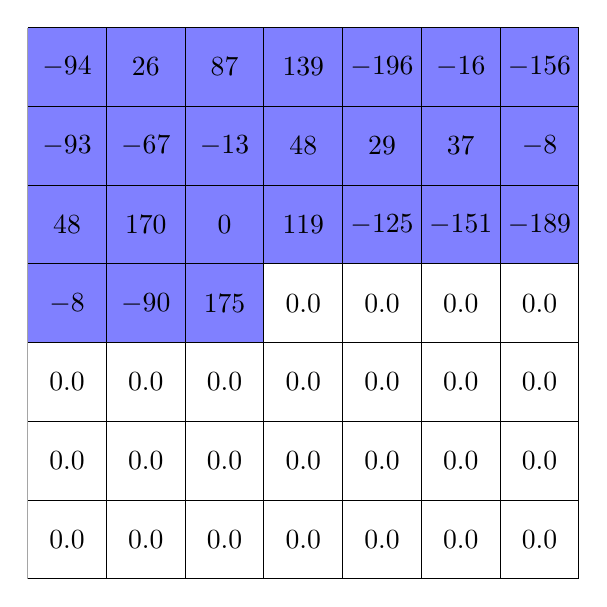
\begin{tikzpicture}

\clip (0, 0) rectangle (7, 7);

\fill[white!50!blue] (0, 4) rectangle (7, 7);
\fill[white!50!blue] (0, 3) rectangle (3, 4);

\draw[step=1] (0, 0) grid (7, 7);

\foreach \x in {0.5, 1.5, ..., 6.5}{
	\foreach \y in {0.5, 1.5, 2.5}{
		\node at (\x, \y) {0.0};
	}
}
\foreach \x in {3.5, 4.5, 5.5, 6.5}{
	\node at (\x, 3.5) {0.0};
}
\foreach \x in {0.5, 1.5, 2.5}{
	\node at (\x, 3.5) { $ \pgfmathrandom{-200, 200} \myround{\pgfmathresult} $ };
}
\foreach \x in {0.5, 1.5, ..., 6.5}{
	\foreach \y in {4.5, 5.5, 6.5}{
		\node at (\x, \y) { $ \pgfmathrandom{-200, 200} \myround{\pgfmathresult} $ };
	}
}

\end{tikzpicture}
\end{document}
